\begin{figure}[htbp]
	\centering
	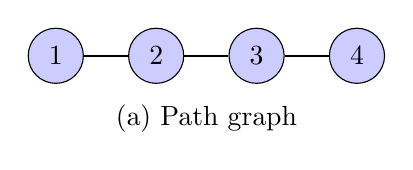
\begin{tikzpicture}[scale=0.85]
		\node[draw, circle, fill=blue!20, minimum size=0.7cm] (1) at (0,0) {1};
		\node[draw, circle, fill=blue!20, minimum size=0.7cm] (2) at (1.5,0) {2};
		\node[draw, circle, fill=blue!20, minimum size=0.7cm] (3) at (3,0) {3};
		\node[draw, circle, fill=blue!20, minimum size=0.7cm] (4) at (4.5,0) {4};
		\draw[thick] (1) -- (2) -- (3) -- (4);
		\node[below=0.5cm] at (2.25,0) {(a) Path graph};
	\end{tikzpicture}

	\vspace{0.5cm}

	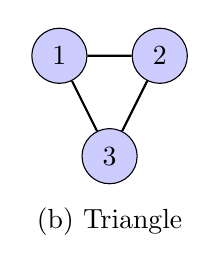
\begin{tikzpicture}[scale=0.85]
		\node[draw, circle, fill=blue!20, minimum size=0.7cm] (c1) at (0,1) {1};
		\node[draw, circle, fill=blue!20, minimum size=0.7cm] (c2) at (1.5,1) {2};
		\node[draw, circle, fill=blue!20, minimum size=0.7cm] (c3) at (0.75,-0.5) {3};
		\draw[thick] (c1) -- (c2) -- (c3) -- (c1);
		\node[below=1.8cm] at (0.75,1) {(b) Triangle};
	\end{tikzpicture}

	\vspace{0.5cm}

	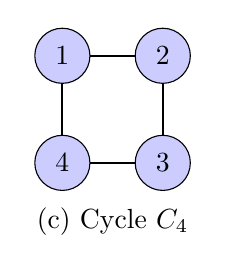
\begin{tikzpicture}[scale=0.85]
		\node[draw, circle, fill=blue!20, minimum size=0.7cm] (s1) at (0,0.8) {1};
		\node[draw, circle, fill=blue!20, minimum size=0.7cm] (s2) at (1.5,0.8) {2};
		\node[draw, circle, fill=blue!20, minimum size=0.7cm] (s3) at (1.5,-0.8) {3};
		\node[draw, circle, fill=blue!20, minimum size=0.7cm] (s4) at (0,-0.8) {4};
		\draw[thick] (s1) -- (s2) -- (s3) -- (s4) -- (s1);
		\node[below=1.8cm] at (0.75,0.8) {(c) Cycle $C_4$};


	\end{tikzpicture}

	\vspace{0.3cm}
	\caption{Different graph representations of the GHZ state. The GHZ state can be represented as a path graph, cycle graph, or other connected structures, all of which are locally complemented to each other and thus share equivalent entanglement properties.}
	\label{fig:ghz-graph-equivalence}
\end{figure}
